\documentclass{article}
\usepackage{graphicx}
\usepackage{subcaption}
\begin{document}
	\section{Motivation}
	The programming language is python. The basic algorithm is the nearest centroid mean algorithm. The algorithm initially compute the mean for each class. The mean is a vector which is computed by averaging all features of training data. The algorithm compute the Euclidean distance between vector of mean trained by the classifier and vector of test data. 
	\section{Problem solution}
	\subsection{problem a}
	Two figures is generated by using \textit{PlotDecBoundaries()}. The CSV file 
	\begin{figure}[hbt!]
		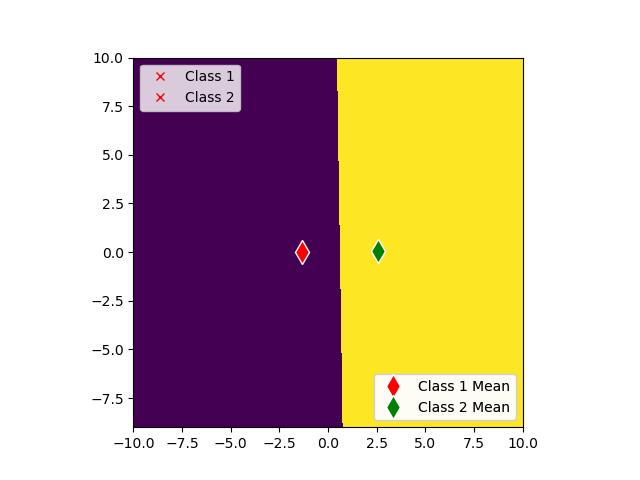
\includegraphics[width=\linewidth]{images/synthetic1.png}
		\caption{synthetic1}
		\label{fig:synthetic1}
	\end{figure}
The Figure \ref{fig:synthetic1} shows the boundary is horizontal 
	\begin{figure}[hbt!]
		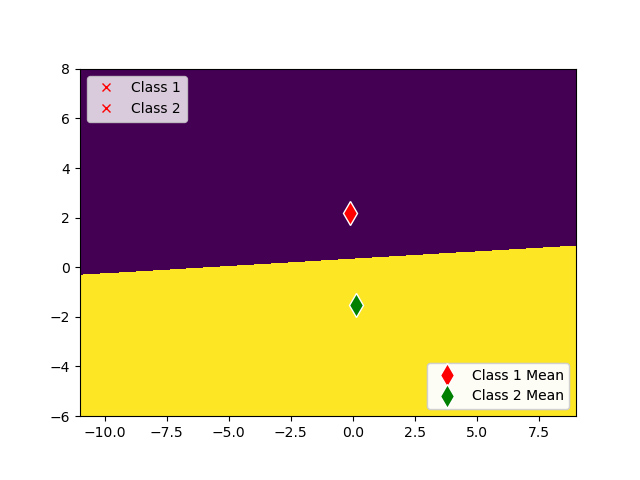
\includegraphics[width=\linewidth]{images/synthetic2.png}
		\caption{synthetic2}
		\label{fig:synthetic2}
	\end{figure}
		\begin{table}[hbt!]
		\begin{center}
		\begin{tabular}{| l | l | l | p{5cm} |}
		\hline
			Data      & Error rate & Test samples  \\ \hline
			synthetic1& 0.24        & 100    \\  \hline
			synthetic2& 0.04		& 100    \\   \hline
		\end{tabular}
		\end{center}
	\caption{Error rate}
	\label{table: errorrate}
	\end{table}
sdfsdfs \\
	\subsection{problem b}
The error rate of both synthetic data set is the same.  
	\section{Summary}
	
\end{document}